\documentclass[10pt,twocolumn,letterpaper]{article}

\usepackage{relsize}
\usepackage{fg}
\usepackage{times}
\usepackage{epsfig}
\usepackage{graphicx}
\usepackage{amsmath}
\usepackage{amssymb}
\usepackage{bm}
\usepackage{textcomp}
\renewcommand*{\d}{\mathrm{d}}
\newcommand*{\dd}{\partial}
\newcommand*{\diffp}[2]{\ensuremath{\frac{\dd #1}{\dd #2}}}
\newcommand*{\diffpp}[3]{\ensuremath{\frac{\dd^2 #1}{\dd #2 \dd #3}}}
\newcommand*{\diffppp}[4]{\ensuremath{\frac{\dd^3 #1}{\dd #2 \dd #3 \dd #4}}}
\newcommand*{\difff}[2]{\ensuremath{\frac{\d #1}{\d #2}}}
\newcommand*{\diffff}[3]{\ensuremath{\frac{\d^2 #1}{\d #2 \d #3}}}
\newcommand*{\difffp}[3]{\ensuremath{\frac{\dd\d #1}{\d #2 \dd #3}}}
\newcommand*{\difffpp}[4]{\ensuremath{\frac{\dd^2\d #1}{\d #2 \dd #3 \dd #4}}}

\newcommand{\Matrix}[1]{\begin{bmatrix} #1 \end{bmatrix}}
\newcommand{\Vector}[1]{\Matrix{#1}}
\newcommand*{\SET}[1]  {\ensuremath{\mathcal{#1}}}
\newcommand*{\MAT}[1]  {\ensuremath{\mathbf{#1}}}
\newcommand*{\VEC}[1]  {\ensuremath{\bm{#1}}}
\newcommand*{\CONST}[1]{\ensuremath{\mathit{#1}}}
\newcommand*{\norm}[1]{\mathopen\| #1 \mathclose\|}% use instead of $\|x\|$
\newcommand*{\abs}[1]{\mathopen| #1 \mathclose|}% use instead of $\|x\|$
\newcommand*{\absLR}[1]{\left| #1 \right|}% use instead of $\|x\|$
\newcommand*{\normLR}[1]{\left\| #1 \right\|}% use instead of $\|x\|$
% Include other packages here, before hyperref.

% If you comment hyperref and then uncomment it, you should delete
% egpaper.aux before re-running latex.  (Or just hit 'q' on the first latex
% run, let it finish, and you should be clear).
\usepackage[pagebackref=true,breaklinks=true,letterpaper=true,colorlinks,bookmarks=false]{hyperref}


\fgfinalcopy % *** Uncomment this line for the final submission

\def\httilde{\mbox{\tt\raisebox{-.5ex}{\symbol{126}}}}

% Pages are numbered in submission mode, and unnumbered in camera-ready
\iffgfinal\pagestyle{empty}\fi
\begin{document}

%%%%%%%%% TITLE
\title{Expression Invariant 3D Face Recognition with a Morphable Model}

\author{Brian Amberg\\
{\tt\small brian.amberg@unibas.ch} \and
Reinhard Knothe\\
{\tt\small reinhard.knothe@unibas.ch} \and
Thomas Vetter\\
{\tt\small thomas.vetter@unibas.ch} 
}

\maketitle
% \thispagestyle{empty}

%%%%%%%%% ABSTRACT
\begin{abstract}
  We present an expression-invariant method for face recognition by fitting an
  identity/expression separated 3D Morphable Model to shape data. The
  expression model greatly improves recognition and retrieval rates in the
  uncooperative setting, while achieving recognition rates on par with the best
  recognition algorithms in the face recognition great vendor test. The
  fitting is performed with a robust nonrigid ICP algorithm. It is able to
  perform face recognition in a fully automated scenario and on noisy data.
  The system was evaluated on two datasets, one
  with a high noise level and strong expressions, and the standard UND range
  scan database, showing that while expression invariance increases recognition
  and retrieval performance for the expression dataset, it does not decrease
  performance on the neutral dataset. The high recognition rates are achieved
  even with a purely shape based method, without taking image data into
  account.
\end{abstract}

%%%%%%%%% BODY TEXT
\section{Introduction}
We present a system which is using shape information from a 3D scanner to
perform automated face recognition. The main novelty of the system is its
invariance to expressions. The system is tested on two
public datasets. It is fully automatic and can handle the typical artifacts of
3D scanners, namely outliers and missing regions. Face recognition in this
setting is a difficult task, and difficult tasks benefit from strong prior knowledge.
To introduce the prior knowledge we use a 3D Morphable Model
(3DMM)~\cite{blanz:model}, which is a generative statistical model of 3D faces.
3DMMs have been applied successfully for face recognition on different
modalities. The most challenging setting is recognition from single images
under varying light and illumination.  This was adressed
by~\cite{blanz03:face_rec,romdhani:recognition}. There, a 3DMM with shape,
texture and illumination model was fit to probe and gallery images.  As the
model separates shape and albedo parameters from pose and lighting, it enables
pose and lighting-invariant recognition. We use the same idea for
expression-invariant face recognition from 3D shape. We fit an identity/expression
separating
3DMM~\cite{blanz03:expression} to shape data and normalize the
resulting face by removing the pose and expression components. See
Figure~\ref{fig:fitting} for an example of expression normalization. The
expression and pose normalized data allows then efficient and effective
recognition. A 3D MM has been fitted to range data before~\cite{blanz07:range}
and the results were even evaluated on part of the UND database. Our approach
differs from this work in the fitting method employed, which is independent of
the acquisition device, and in the use of an expression model to improve face
recognition. Additionally, our method is fully automatic,
while~\cite{blanz07:range} needed seven manually selected landmarks.

\begin{figure}
  \vspace{-0.5em}
  \begin{tabular}{@{ }c@{ }c@{ }c@{ }c@{}}
    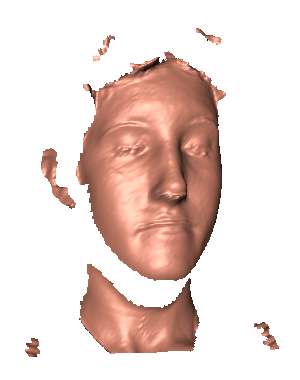
\includegraphics[height=0.42\linewidth]{16_1_tgt}&
    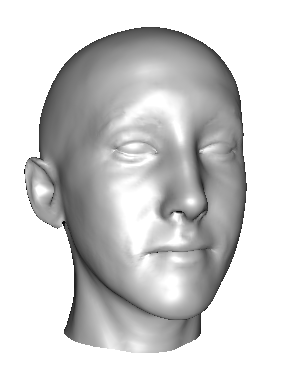
\includegraphics[height=0.42\linewidth]{16_1_expression}&
    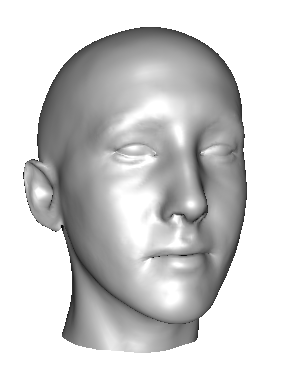
\includegraphics[height=0.42\linewidth]{16_1_neutral}\\[-0.8em]
    \smaller a) Target & \smaller b) Fit & \smaller c) Normalized\\[0.8em]
    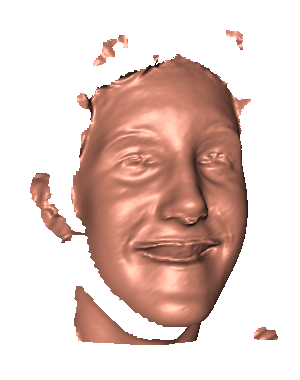
\includegraphics[height=0.42\linewidth]{16_6_tgt}&
    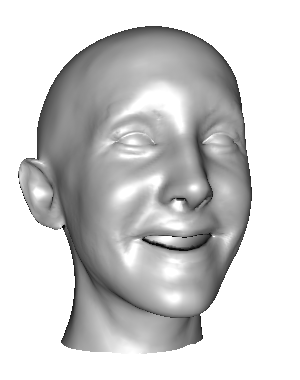
\includegraphics[height=0.42\linewidth]{16_6_expression}&
    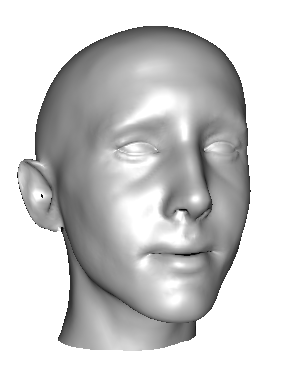
\includegraphics[height=0.42\linewidth]{16_6_neutral}\\[-0.8em]
    \smaller a) Target & \smaller b) Fit & \smaller c) Normalized
  \end{tabular}
  \vspace{0.5em}
  \caption{Expression normalisation for two scans of the same individual.  
  The robust fitting gives a good estimate (b) of the true face surface given
  the noisy measurement (a). It fills in holes and removes artifacts using
  prior knowledge from the face model. The pose and expression normalized faces
  (c) are used for face recognition.
  }
  \label{fig:fitting}
\end{figure}
Expression-invariant recognition for shape data was also approached in
\cite{xiaoguang06:face_matching}, where a person specific 3D Morphable
Expression Model was learned for each subject in the gallery. In contrast, we
are using a general 3DMM learned from an independent database of face shapes
which can be applied without any relearning to a new scan. This makes the
enrollment phase trivial and the recognition phase effectively constant in the
size of the gallery while still being accurate. We have to fit just one
model to the probe, which can then be compared efficiently to
the enrolled subjects, by comparing their coefficients in the low dimensional
face space. While the number of comparisions is still at most linear in the
number of examples (and can be made sublinear with an indexing method) the time
it takes to compare coefficients in face space is neglectible compared to
fitting time.
%
Model-less approaches which align the probe to each example in the database
using e.g.\ ICP~\cite{bowyer05:icp_recognition} suffer from the same problem
as~\cite{xiaoguang06:face_matching}.
Because the probe has to be aligned with each gallery scan these methods scale
linearly in the gallery size, While our model based approach needs only a
single fit to the probe.

Another interesting model-less approach~\cite{bronstein05:face_rec} compares
surface by the distribution of geodesics, which stays constant for nonrigidly
deforming (but not stretching or tearing) objects.  This approach is difficult
to apply in this setting though, as the scanning produces holes, disconnected
regions and strong noise, which can best be handled by a method which uses
specific information about the object class.
			  
\section{Model}
A PCA model~\cite{blanz:model} built from 175 subjects was used. It was build
from one neutral expression face scan per identity and 50 expression scans of a
subset of the subjects. The data was registered with a modification
of~\cite{amberg07:nicp}.
The identity model consists of a mean shape $\VEC\mu$ and a matrix of offset
vectors $\MAT M_n$ such that a new face instance $\VEC f$ is generated from a
vector of coefficients $\VEC\alpha_n$ as
\begin{align}
  \VEC f&=\VEC\mu + \MAT M_n\VEC\alpha_n\qquad.
\end{align}
The model is constructed such that the $\alpha_i$ are independently normally
distributed with zero mean and unit variance under the standard assumption of a
Gaussian distribution of the data. This was done by performing PCA
on the data matrix built from the mean free shape vectors.
Additionally, for each of the 50 expression scans, we calculated an expression
vector as the difference between the expression scan and the corresponding
neutral scan of that subject.
This data is already mode-centered, if we regard the neutral
expression as the natural mode of expression data. On these offset vectors
again PCA was applied to get an expression matrix $\MAT M_e$ and 
expression coefficients $\VEC\alpha_e$, such that the complete expression model is
\begin{align}
  \VEC f&=\VEC\mu + \MAT M_n\VEC\alpha_n + \MAT M_e\VEC\alpha_e
         =\VEC\mu + \MAT M\VEC\alpha\qquad,\\
  \MAT M &= \Matrix{\MAT M_n &|& \MAT M_e} \qquad \VEC\alpha = \Matrix{\VEC\alpha_n \\ \VEC\alpha_e}\qquad.
\end{align}
The basic assumption of this paper is, that the face and expression space are
linearly independent, such that each face is represented by a unique set of
coefficients.  While the resulting expression and identity matrices are not
perfectly orthogonal, they do have little overlap, which together with the
regularisation employed is sufficient for this application. We assume, that the
overlap between the spaces is due to the fact that it is impossible to aquire
perfectly consistent neutral expressions.

We use the registered scans and a mirrored version of each registered scan to
increase the variability of the model. This allows us to calculate a model with
more than 175 neutral coefficients.

\section{Fitting}
The fitting algorithm used in this paper is a variant of the nonrigid ICP work
in~\cite{amberg07:nicp}. The main difference, is that the deformation model is
a statistical model and the optimisation in each step is an iterative method,
which finds the minimum of a convex function. Additionally, as it is applied on
noisy data (see Figure~\ref{fig:difficult}), we included a more elaborate robust weighting term.  Like other
ICP methods, it is a local optimization method, which does not guarantee
convergence to the global mimimum, but is dependent on the initialization. It
consists of the following steps
\begin{itemize}
  \item Iterate over regularization values $\theta_1>\dots>\theta_N$:
  \begin{itemize}
  \item Repeat until convergence:
    \begin{enumerate}
    \item Find candidate correspondences by searching for the closest compatible
      point for each model vertex.
    \item Weight the correspondences by their distance using a robust estimator.
    \item Fit the 3DMM to these correspondences using a
      regularization strength of $\theta_i$\label{step_fit}.
    \item Continue with the lower $\theta_{i+1}$ if the median change in vertex
      position is smaller than a threshold.
    \end{enumerate}
  \end{itemize}
\end{itemize}
\begin{figure}
  \vspace{-1.0em}
  \begin{tabular}{@{ }c@{ }c@{ }c@{ }c@{}}
    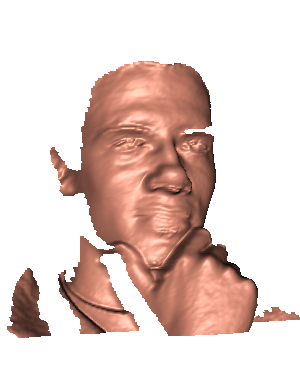
\includegraphics[height=0.42\linewidth]{56_4_tgt}&
    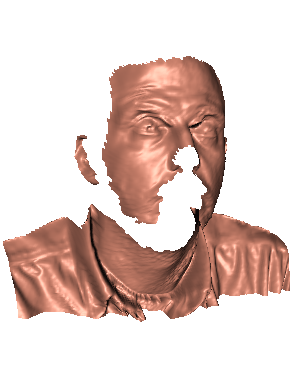
\includegraphics[height=0.42\linewidth]{23_2_tgt}&
    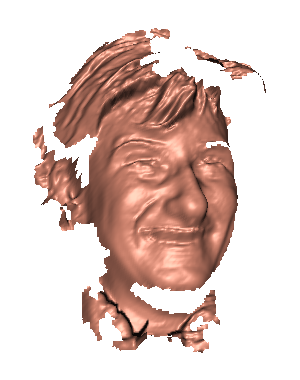
\includegraphics[height=0.42\linewidth]{5_6_tgt}\\[-1.0em]
                       & \smaller a) Targets & \\[0.2em]
    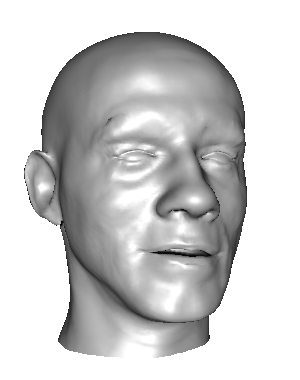
\includegraphics[height=0.42\linewidth]{56_4_expression}&
    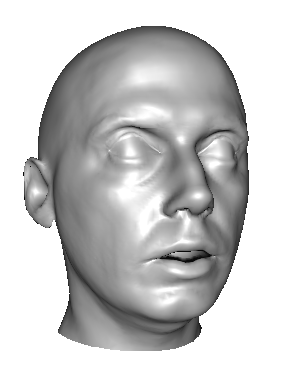
\includegraphics[height=0.42\linewidth]{23_2_expression}& 
    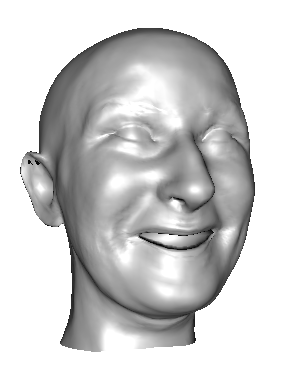
\includegraphics[height=0.42\linewidth]{5_6_expression}\\[-0.8em]
                    & \smaller b) Fits & 
  \end{tabular}
  \vspace{0.2em}
  \caption{The reconstruction (b) is robust against scans (a) with artifacts, noise, and holes.}
  \label{fig:difficult}
\end{figure}
The search for the closest compatible point takes only points into account which
have conforming normals, are closer than a threshold, and are not on or close
to the border of the scan. This has the effect of removing many outliers.  The
search is sped up by organizing the target scan in a space partitioning tree
made up of spheres.
The correspondences are then weighted with a robust function by their
residual distance. The robust function is linear for distances smaller than
$2$mm, behaves like $1/x$ between $2$mm and
$20$mm, and is zero for a distance larger than $20$mm.
Note, that it is necessary to balance robustness and regularization, as the
right balance depends on the noise characteristic of the data. Suitable values
were determined manually from a few scans of the GavabDB database and kept
constant for all experiments as well on the GavaDB as on the UND database.  In
step~\ref{step_fit} the 3DMM is fit to 3D-3D point correspondences.  This is
done with a gauss-newton least squares optimization, using an analytic Jacobian
and Gauss-Newton Hessian approximation.  Denote the correspondence points by
$\MAT u=\Matrix{\VEC u_1, \dots, \VEC u_n}$ and the rows of the model which
correspond to the $i$th vertex by subscript $i$, then we can write the cost
function mimized in this step as
\begin{align}
  f(\MAT R, \VEC t, \VEC\alpha) &= \sum_i \normLR{\MAT R( \VEC\mu_i + \MAT M_i\VEC\alpha) + \VEC t - \VEC u_i}^2 + \lambda\normLR{\VEC\alpha}^2\qquad.\label{eqn:mincost}
\end{align}
%We make the norm dependent on the target normal by  using an orthonormal
%covariance matrix $\MAT C_i$ per vertex, which makes the cost of deviation
%along the normal higher than deviations inside the target surface. 
%\begin{align}
%  \MAT C_i &= \Matrix{ \VEC n_i^T\\ \nu \VEC a_i^T\\\nu\VEC b_i^T} & \VEC n_i &\bot \VEC a_i \bot \VEC b_i \bot \VEC n_i
%\end{align}
%where $\VEC n_i$ is the normal of the target correspondence and $\nu$ is an
%anisotropy parameter. If we do not use the anisotropic distance measure (i.e.
%$\MAT C_i=\MAT I$), then the cost function Equation~\ref{eqn:mincost} can be
%minimized more efficiently by changing it to
This can be minimized more efficiently by changing the direction of the rigid transform to
\begin{align}
  f(\MAT R, \VEC t, \VEC\alpha) &= \sum_i \normLR{ \VEC\mu_i + \MAT M_i\VEC\alpha + {\VEC t'} - {\MAT R'}\VEC u_i }^2 + \lambda\normLR{\VEC\alpha}^2\nonumber\\
  {\VEC t'} &= \MAT R^{-1}\VEC t\qquad {\MAT R'} = \MAT R^{-1}\qquad.
\end{align}
because then the Jacobian consists of a large constant part and three columns
which depend on the iteration.
\begin{align}
  F_i &= \VEC\mu_i + \MAT M_i\VEC\alpha + {\VEC t'} - {\MAT R'_{r_1,r_2,r_3}}\VEC u_i\\
  \diffp{F_i}{\VEC\alpha} &= \MAT M_i\qquad
  \diffp{F_i}{\VEC t'} = \MAT I_3\qquad
  \diffp{F_i}{r_i} = \diffp{\MAT R'_{r_1,r_2,r_3}}{r_i}\VEC u_i\\
  \MAT J &= \Matrix{\MAT J_c & | & \MAT J_d }\\
  \MAT J_c &= \Matrix{\MAT M & \VEC 1 \otimes \MAT I_3\\ \MAT I & \MAT 0}\\
  \MAT J_d &= \Matrix{(\MAT I \otimes \diffp{\MAT R'}{r_1})\MAT u^T & (\MAT I \otimes \diffp{\MAT R'}{r_2})\MAT u^T& (\MAT I \otimes \diffp{\MAT R'}{r_3})\MAT u^T\\\MAT 0 & \MAT 0 & \MAT 0}
\end{align}
Accordingly, the Hessian can be approximated as
\begin{align}
  \MAT H &= \Matrix{
    \MAT J_c^T\MAT J_c & (\MAT J_c^T\MAT J_d)^T\\
    \MAT J_c^T\MAT J_d & \MAT J_d^T\MAT J_d
  }\qquad.
\end{align}
By precalculating the constant parts of the matrices we can remove most of the
computation time, making step~\ref{step_fit} very fast.

We initialize the registration by locating the tip of the nose with a
heuristic, which assumes that the head is upright and looking into the camera.
This initialization is good enough to for a fully automatic
fit, as the fitting behaves like rigid ICP in the beginning, and rigid ICP is
known to have a large basin of convergence.

\section{Experiments}
\begin{figure*}
  \begin{tabular}{cc}
    \scalebox{0.82}{\input{shrec_MNCG}} &
    \scalebox{0.82}{\input{und_MNCG}}
  \end{tabular}
  \caption{For the expression dataset the retrieval rate is improved by
  including the expression model, while for the neutral expression dataset the
  performance does not decrease. Plotted is the mean normalized cumulative
  gain, which is the number of retrieved correct answers divided by the number
  of possible correct answers. Note also the different scales of the MNCG
  curves for the two datasets. Our approach has a high accuracy on the
  neutral (UND) dataset.}
  \label{fig:mcg}
\end{figure*}
\begin{figure*}
  \begin{tabular}{cc}
    \scalebox{0.82}{% GNUPLOT: LaTeX picture with Postscript
\begingroup
  \fontfamily{phv}%
  \selectfont
  \makeatletter
  \providecommand\color[2][]{%
    \GenericError{(gnuplot) \space\space\space\@spaces}{%
      Package color not loaded in conjunction with
      terminal option `colourtext'%
    }{See the gnuplot documentation for explanation.%
    }{Either use 'blacktext' in gnuplot or load the package
      color.sty in LaTeX.}%
    \renewcommand\color[2][]{}%
  }%
  \providecommand\includegraphics[2][]{%
    \GenericError{(gnuplot) \space\space\space\@spaces}{%
      Package graphicx or graphics not loaded%
    }{See the gnuplot documentation for explanation.%
    }{The gnuplot epslatex terminal needs graphicx.sty or graphics.sty.}%
    \renewcommand\includegraphics[2][]{}%
  }%
  \providecommand\rotatebox[2]{#2}%
  \@ifundefined{ifGPcolor}{%
    \newif\ifGPcolor
    \GPcolortrue
  }{}%
  \@ifundefined{ifGPblacktext}{%
    \newif\ifGPblacktext
    \GPblacktextfalse
  }{}%
  % define a \g@addto@macro without @ in the name:
  \let\gplgaddtomacro\g@addto@macro
  % define empty templates for all commands taking text:
  \gdef\gplbacktext{}%
  \gdef\gplfronttext{}%
  \makeatother
  \ifGPblacktext
    % no textcolor at all
    \def\colorrgb#1{}%
    \def\colorgray#1{}%
  \else
    % gray or color?
    \ifGPcolor
      \def\colorrgb#1{\color[rgb]{#1}}%
      \def\colorgray#1{\color[gray]{#1}}%
      \expandafter\def\csname LTw\endcsname{\color{white}}%
      \expandafter\def\csname LTb\endcsname{\color{black}}%
      \expandafter\def\csname LTa\endcsname{\color{black}}%
      \expandafter\def\csname LT0\endcsname{\color[rgb]{1,0,0}}%
      \expandafter\def\csname LT1\endcsname{\color[rgb]{0,1,0}}%
      \expandafter\def\csname LT2\endcsname{\color[rgb]{0,0,1}}%
      \expandafter\def\csname LT3\endcsname{\color[rgb]{1,0,1}}%
      \expandafter\def\csname LT4\endcsname{\color[rgb]{0,1,1}}%
      \expandafter\def\csname LT5\endcsname{\color[rgb]{1,1,0}}%
      \expandafter\def\csname LT6\endcsname{\color[rgb]{0,0,0}}%
      \expandafter\def\csname LT7\endcsname{\color[rgb]{1,0.3,0}}%
      \expandafter\def\csname LT8\endcsname{\color[rgb]{0.5,0.5,0.5}}%
    \else
      % gray
      \def\colorrgb#1{\color{black}}%
      \def\colorgray#1{\color[gray]{#1}}%
      \expandafter\def\csname LTw\endcsname{\color{white}}%
      \expandafter\def\csname LTb\endcsname{\color{black}}%
      \expandafter\def\csname LTa\endcsname{\color{black}}%
      \expandafter\def\csname LT0\endcsname{\color{black}}%
      \expandafter\def\csname LT1\endcsname{\color{black}}%
      \expandafter\def\csname LT2\endcsname{\color{black}}%
      \expandafter\def\csname LT3\endcsname{\color{black}}%
      \expandafter\def\csname LT4\endcsname{\color{black}}%
      \expandafter\def\csname LT5\endcsname{\color{black}}%
      \expandafter\def\csname LT6\endcsname{\color{black}}%
      \expandafter\def\csname LT7\endcsname{\color{black}}%
      \expandafter\def\csname LT8\endcsname{\color{black}}%
    \fi
  \fi
  \setlength{\unitlength}{0.0500bp}%
  \begin{picture}(5760.00,2520.00)%
    \gplgaddtomacro\gplbacktext{%
      \csname LTb\endcsname%
      \put(810,540){\makebox(0,0)[r]{\strut{} 0}}%
      \csname LTb\endcsname%
      \put(810,828){\makebox(0,0)[r]{\strut{} 0.2}}%
      \csname LTb\endcsname%
      \put(810,1116){\makebox(0,0)[r]{\strut{} 0.4}}%
      \csname LTb\endcsname%
      \put(810,1404){\makebox(0,0)[r]{\strut{} 0.6}}%
      \csname LTb\endcsname%
      \put(810,1692){\makebox(0,0)[r]{\strut{} 0.8}}%
      \csname LTb\endcsname%
      \put(810,1980){\makebox(0,0)[r]{\strut{} 1}}%
      \csname LTb\endcsname%
      \put(918,360){\makebox(0,0){\strut{} 0}}%
      \csname LTb\endcsname%
      \put(1825,360){\makebox(0,0){\strut{} 0.2}}%
      \csname LTb\endcsname%
      \put(2732,360){\makebox(0,0){\strut{} 0.4}}%
      \csname LTb\endcsname%
      \put(3640,360){\makebox(0,0){\strut{} 0.6}}%
      \csname LTb\endcsname%
      \put(4547,360){\makebox(0,0){\strut{} 0.8}}%
      \csname LTb\endcsname%
      \put(5454,360){\makebox(0,0){\strut{} 1}}%
      \put(180,1260){\rotatebox{90}{\makebox(0,0){\strut{}Precision}}}%
      \put(3186,90){\makebox(0,0){\strut{}Recall}}%
      \put(3186,2250){\makebox(0,0){\strut{}GavabDB: Precision Recall}}%
    }%
    \gplgaddtomacro\gplfronttext{%
      \csname LTb\endcsname%
      \put(2754,873){\makebox(0,0)[r]{\strut{}neutral model}}%
      \csname LTb\endcsname%
      \put(2754,693){\makebox(0,0)[r]{\strut{}expression model}}%
    }%
    \gplbacktext
    \put(0,0){\includegraphics{shrec_PR}}%
    \gplfronttext
  \end{picture}%
\endgroup
} &
    \scalebox{0.82}{% GNUPLOT: LaTeX picture with Postscript
\begingroup
  \fontfamily{phv}%
  \selectfont
  \makeatletter
  \providecommand\color[2][]{%
    \GenericError{(gnuplot) \space\space\space\@spaces}{%
      Package color not loaded in conjunction with
      terminal option `colourtext'%
    }{See the gnuplot documentation for explanation.%
    }{Either use 'blacktext' in gnuplot or load the package
      color.sty in LaTeX.}%
    \renewcommand\color[2][]{}%
  }%
  \providecommand\includegraphics[2][]{%
    \GenericError{(gnuplot) \space\space\space\@spaces}{%
      Package graphicx or graphics not loaded%
    }{See the gnuplot documentation for explanation.%
    }{The gnuplot epslatex terminal needs graphicx.sty or graphics.sty.}%
    \renewcommand\includegraphics[2][]{}%
  }%
  \providecommand\rotatebox[2]{#2}%
  \@ifundefined{ifGPcolor}{%
    \newif\ifGPcolor
    \GPcolortrue
  }{}%
  \@ifundefined{ifGPblacktext}{%
    \newif\ifGPblacktext
    \GPblacktextfalse
  }{}%
  % define a \g@addto@macro without @ in the name:
  \let\gplgaddtomacro\g@addto@macro
  % define empty templates for all commands taking text:
  \gdef\gplbacktext{}%
  \gdef\gplfronttext{}%
  \makeatother
  \ifGPblacktext
    % no textcolor at all
    \def\colorrgb#1{}%
    \def\colorgray#1{}%
  \else
    % gray or color?
    \ifGPcolor
      \def\colorrgb#1{\color[rgb]{#1}}%
      \def\colorgray#1{\color[gray]{#1}}%
      \expandafter\def\csname LTw\endcsname{\color{white}}%
      \expandafter\def\csname LTb\endcsname{\color{black}}%
      \expandafter\def\csname LTa\endcsname{\color{black}}%
      \expandafter\def\csname LT0\endcsname{\color[rgb]{1,0,0}}%
      \expandafter\def\csname LT1\endcsname{\color[rgb]{0,1,0}}%
      \expandafter\def\csname LT2\endcsname{\color[rgb]{0,0,1}}%
      \expandafter\def\csname LT3\endcsname{\color[rgb]{1,0,1}}%
      \expandafter\def\csname LT4\endcsname{\color[rgb]{0,1,1}}%
      \expandafter\def\csname LT5\endcsname{\color[rgb]{1,1,0}}%
      \expandafter\def\csname LT6\endcsname{\color[rgb]{0,0,0}}%
      \expandafter\def\csname LT7\endcsname{\color[rgb]{1,0.3,0}}%
      \expandafter\def\csname LT8\endcsname{\color[rgb]{0.5,0.5,0.5}}%
    \else
      % gray
      \def\colorrgb#1{\color{black}}%
      \def\colorgray#1{\color[gray]{#1}}%
      \expandafter\def\csname LTw\endcsname{\color{white}}%
      \expandafter\def\csname LTb\endcsname{\color{black}}%
      \expandafter\def\csname LTa\endcsname{\color{black}}%
      \expandafter\def\csname LT0\endcsname{\color{black}}%
      \expandafter\def\csname LT1\endcsname{\color{black}}%
      \expandafter\def\csname LT2\endcsname{\color{black}}%
      \expandafter\def\csname LT3\endcsname{\color{black}}%
      \expandafter\def\csname LT4\endcsname{\color{black}}%
      \expandafter\def\csname LT5\endcsname{\color{black}}%
      \expandafter\def\csname LT6\endcsname{\color{black}}%
      \expandafter\def\csname LT7\endcsname{\color{black}}%
      \expandafter\def\csname LT8\endcsname{\color{black}}%
    \fi
  \fi
  \setlength{\unitlength}{0.0500bp}%
  \begin{picture}(5760.00,2520.00)%
    \gplgaddtomacro\gplbacktext{%
      \csname LTb\endcsname%
      \put(810,540){\makebox(0,0)[r]{\strut{} 0}}%
      \csname LTb\endcsname%
      \put(810,828){\makebox(0,0)[r]{\strut{} 0.2}}%
      \csname LTb\endcsname%
      \put(810,1116){\makebox(0,0)[r]{\strut{} 0.4}}%
      \csname LTb\endcsname%
      \put(810,1404){\makebox(0,0)[r]{\strut{} 0.6}}%
      \csname LTb\endcsname%
      \put(810,1692){\makebox(0,0)[r]{\strut{} 0.8}}%
      \csname LTb\endcsname%
      \put(810,1980){\makebox(0,0)[r]{\strut{} 1}}%
      \csname LTb\endcsname%
      \put(918,360){\makebox(0,0){\strut{} 0}}%
      \csname LTb\endcsname%
      \put(1825,360){\makebox(0,0){\strut{} 0.2}}%
      \csname LTb\endcsname%
      \put(2732,360){\makebox(0,0){\strut{} 0.4}}%
      \csname LTb\endcsname%
      \put(3640,360){\makebox(0,0){\strut{} 0.6}}%
      \csname LTb\endcsname%
      \put(4547,360){\makebox(0,0){\strut{} 0.8}}%
      \csname LTb\endcsname%
      \put(5454,360){\makebox(0,0){\strut{} 1}}%
      \put(180,1260){\rotatebox{90}{\makebox(0,0){\strut{}Precision}}}%
      \put(3186,90){\makebox(0,0){\strut{}Recall}}%
      \put(3186,2250){\makebox(0,0){\strut{}UND: Precision Recall}}%
    }%
    \gplgaddtomacro\gplfronttext{%
      \csname LTb\endcsname%
      \put(2754,873){\makebox(0,0)[r]{\strut{}neutral model}}%
      \csname LTb\endcsname%
      \put(2754,693){\makebox(0,0)[r]{\strut{}expression model}}%
    }%
    \gplbacktext
    \put(0,0){\includegraphics{und_PR}}%
    \gplfronttext
  \end{picture}%
\endgroup
}
  \end{tabular}
  \caption{Use of the expression model improves retrieval performance.
  Plotted are precision and recall for different retrieval depths. The lower
  precision of the UND database is due to the fact that some queries have no
  correct answers. For the UND database we achieve total recall when querying
  nine answers, while the maximal number of scans per individual is eight,
  while for the GavabDB database the expression model gives a strong
    improvement in recall rate but full recall can not be achieved.}
  \label{fig:precision_expression}
\end{figure*}

\begin{figure*}
  \begin{tabular}{cc}
    \scalebox{0.82}{% GNUPLOT: LaTeX picture with Postscript
\begingroup
  \fontfamily{phv}%
  \selectfont
  \makeatletter
  \providecommand\color[2][]{%
    \GenericError{(gnuplot) \space\space\space\@spaces}{%
      Package color not loaded in conjunction with
      terminal option `colourtext'%
    }{See the gnuplot documentation for explanation.%
    }{Either use 'blacktext' in gnuplot or load the package
      color.sty in LaTeX.}%
    \renewcommand\color[2][]{}%
  }%
  \providecommand\includegraphics[2][]{%
    \GenericError{(gnuplot) \space\space\space\@spaces}{%
      Package graphicx or graphics not loaded%
    }{See the gnuplot documentation for explanation.%
    }{The gnuplot epslatex terminal needs graphicx.sty or graphics.sty.}%
    \renewcommand\includegraphics[2][]{}%
  }%
  \providecommand\rotatebox[2]{#2}%
  \@ifundefined{ifGPcolor}{%
    \newif\ifGPcolor
    \GPcolortrue
  }{}%
  \@ifundefined{ifGPblacktext}{%
    \newif\ifGPblacktext
    \GPblacktextfalse
  }{}%
  % define a \g@addto@macro without @ in the name:
  \let\gplgaddtomacro\g@addto@macro
  % define empty templates for all commands taking text:
  \gdef\gplbacktext{}%
  \gdef\gplfronttext{}%
  \makeatother
  \ifGPblacktext
    % no textcolor at all
    \def\colorrgb#1{}%
    \def\colorgray#1{}%
  \else
    % gray or color?
    \ifGPcolor
      \def\colorrgb#1{\color[rgb]{#1}}%
      \def\colorgray#1{\color[gray]{#1}}%
      \expandafter\def\csname LTw\endcsname{\color{white}}%
      \expandafter\def\csname LTb\endcsname{\color{black}}%
      \expandafter\def\csname LTa\endcsname{\color{black}}%
      \expandafter\def\csname LT0\endcsname{\color[rgb]{1,0,0}}%
      \expandafter\def\csname LT1\endcsname{\color[rgb]{0,1,0}}%
      \expandafter\def\csname LT2\endcsname{\color[rgb]{0,0,1}}%
      \expandafter\def\csname LT3\endcsname{\color[rgb]{1,0,1}}%
      \expandafter\def\csname LT4\endcsname{\color[rgb]{0,1,1}}%
      \expandafter\def\csname LT5\endcsname{\color[rgb]{1,1,0}}%
      \expandafter\def\csname LT6\endcsname{\color[rgb]{0,0,0}}%
      \expandafter\def\csname LT7\endcsname{\color[rgb]{1,0.3,0}}%
      \expandafter\def\csname LT8\endcsname{\color[rgb]{0.5,0.5,0.5}}%
    \else
      % gray
      \def\colorrgb#1{\color{black}}%
      \def\colorgray#1{\color[gray]{#1}}%
      \expandafter\def\csname LTw\endcsname{\color{white}}%
      \expandafter\def\csname LTb\endcsname{\color{black}}%
      \expandafter\def\csname LTa\endcsname{\color{black}}%
      \expandafter\def\csname LT0\endcsname{\color{black}}%
      \expandafter\def\csname LT1\endcsname{\color{black}}%
      \expandafter\def\csname LT2\endcsname{\color{black}}%
      \expandafter\def\csname LT3\endcsname{\color{black}}%
      \expandafter\def\csname LT4\endcsname{\color{black}}%
      \expandafter\def\csname LT5\endcsname{\color{black}}%
      \expandafter\def\csname LT6\endcsname{\color{black}}%
      \expandafter\def\csname LT7\endcsname{\color{black}}%
      \expandafter\def\csname LT8\endcsname{\color{black}}%
    \fi
  \fi
  \setlength{\unitlength}{0.0500bp}%
  \begin{picture}(5760.00,2520.00)%
    \gplgaddtomacro\gplbacktext{%
      \csname LTb\endcsname%
      \put(918,540){\makebox(0,0)[r]{\strut{} 0}}%
      \csname LTb\endcsname%
      \put(918,720){\makebox(0,0)[r]{\strut{} 0.01}}%
      \csname LTb\endcsname%
      \put(918,900){\makebox(0,0)[r]{\strut{} 0.02}}%
      \csname LTb\endcsname%
      \put(918,1080){\makebox(0,0)[r]{\strut{} 0.03}}%
      \csname LTb\endcsname%
      \put(918,1260){\makebox(0,0)[r]{\strut{} 0.04}}%
      \csname LTb\endcsname%
      \put(918,1440){\makebox(0,0)[r]{\strut{} 0.05}}%
      \csname LTb\endcsname%
      \put(918,1620){\makebox(0,0)[r]{\strut{} 0.06}}%
      \csname LTb\endcsname%
      \put(918,1800){\makebox(0,0)[r]{\strut{} 0.07}}%
      \csname LTb\endcsname%
      \put(918,1980){\makebox(0,0)[r]{\strut{} 0.08}}%
      \csname LTb\endcsname%
      \put(1026,360){\makebox(0,0){\strut{} 0}}%
      \csname LTb\endcsname%
      \put(1764,360){\makebox(0,0){\strut{} 0.005}}%
      \csname LTb\endcsname%
      \put(2502,360){\makebox(0,0){\strut{} 0.01}}%
      \csname LTb\endcsname%
      \put(3240,360){\makebox(0,0){\strut{} 0.015}}%
      \csname LTb\endcsname%
      \put(3978,360){\makebox(0,0){\strut{} 0.02}}%
      \csname LTb\endcsname%
      \put(4716,360){\makebox(0,0){\strut{} 0.025}}%
      \csname LTb\endcsname%
      \put(5454,360){\makebox(0,0){\strut{} 0.03}}%
      \put(180,1260){\rotatebox{90}{\makebox(0,0){\strut{}FRR}}}%
      \put(3240,90){\makebox(0,0){\strut{}FAR}}%
      \put(3240,2250){\makebox(0,0){\strut{}GavabDB: Recognition Performance}}%
    }%
    \gplgaddtomacro\gplfronttext{%
      \csname LTb\endcsname%
      \put(4635,1827){\makebox(0,0)[r]{\strut{}neutral model}}%
      \csname LTb\endcsname%
      \put(4635,1647){\makebox(0,0)[r]{\strut{}expression model}}%
    }%
    \gplbacktext
    \put(0,0){\includegraphics{shrec_FARFRR}}%
    \gplfronttext
  \end{picture}%
\endgroup
} &
    \scalebox{0.82}{% GNUPLOT: LaTeX picture with Postscript
\begingroup
  \fontfamily{phv}%
  \selectfont
  \makeatletter
  \providecommand\color[2][]{%
    \GenericError{(gnuplot) \space\space\space\@spaces}{%
      Package color not loaded in conjunction with
      terminal option `colourtext'%
    }{See the gnuplot documentation for explanation.%
    }{Either use 'blacktext' in gnuplot or load the package
      color.sty in LaTeX.}%
    \renewcommand\color[2][]{}%
  }%
  \providecommand\includegraphics[2][]{%
    \GenericError{(gnuplot) \space\space\space\@spaces}{%
      Package graphicx or graphics not loaded%
    }{See the gnuplot documentation for explanation.%
    }{The gnuplot epslatex terminal needs graphicx.sty or graphics.sty.}%
    \renewcommand\includegraphics[2][]{}%
  }%
  \providecommand\rotatebox[2]{#2}%
  \@ifundefined{ifGPcolor}{%
    \newif\ifGPcolor
    \GPcolortrue
  }{}%
  \@ifundefined{ifGPblacktext}{%
    \newif\ifGPblacktext
    \GPblacktextfalse
  }{}%
  % define a \g@addto@macro without @ in the name:
  \let\gplgaddtomacro\g@addto@macro
  % define empty templates for all commands taking text:
  \gdef\gplbacktext{}%
  \gdef\gplfronttext{}%
  \makeatother
  \ifGPblacktext
    % no textcolor at all
    \def\colorrgb#1{}%
    \def\colorgray#1{}%
  \else
    % gray or color?
    \ifGPcolor
      \def\colorrgb#1{\color[rgb]{#1}}%
      \def\colorgray#1{\color[gray]{#1}}%
      \expandafter\def\csname LTw\endcsname{\color{white}}%
      \expandafter\def\csname LTb\endcsname{\color{black}}%
      \expandafter\def\csname LTa\endcsname{\color{black}}%
      \expandafter\def\csname LT0\endcsname{\color[rgb]{1,0,0}}%
      \expandafter\def\csname LT1\endcsname{\color[rgb]{0,1,0}}%
      \expandafter\def\csname LT2\endcsname{\color[rgb]{0,0,1}}%
      \expandafter\def\csname LT3\endcsname{\color[rgb]{1,0,1}}%
      \expandafter\def\csname LT4\endcsname{\color[rgb]{0,1,1}}%
      \expandafter\def\csname LT5\endcsname{\color[rgb]{1,1,0}}%
      \expandafter\def\csname LT6\endcsname{\color[rgb]{0,0,0}}%
      \expandafter\def\csname LT7\endcsname{\color[rgb]{1,0.3,0}}%
      \expandafter\def\csname LT8\endcsname{\color[rgb]{0.5,0.5,0.5}}%
    \else
      % gray
      \def\colorrgb#1{\color{black}}%
      \def\colorgray#1{\color[gray]{#1}}%
      \expandafter\def\csname LTw\endcsname{\color{white}}%
      \expandafter\def\csname LTb\endcsname{\color{black}}%
      \expandafter\def\csname LTa\endcsname{\color{black}}%
      \expandafter\def\csname LT0\endcsname{\color{black}}%
      \expandafter\def\csname LT1\endcsname{\color{black}}%
      \expandafter\def\csname LT2\endcsname{\color{black}}%
      \expandafter\def\csname LT3\endcsname{\color{black}}%
      \expandafter\def\csname LT4\endcsname{\color{black}}%
      \expandafter\def\csname LT5\endcsname{\color{black}}%
      \expandafter\def\csname LT6\endcsname{\color{black}}%
      \expandafter\def\csname LT7\endcsname{\color{black}}%
      \expandafter\def\csname LT8\endcsname{\color{black}}%
    \fi
  \fi
  \setlength{\unitlength}{0.0500bp}%
  \begin{picture}(5760.00,2520.00)%
    \gplgaddtomacro\gplbacktext{%
      \csname LTb\endcsname%
      \put(918,540){\makebox(0,0)[r]{\strut{} 0}}%
      \csname LTb\endcsname%
      \put(918,720){\makebox(0,0)[r]{\strut{} 0.01}}%
      \csname LTb\endcsname%
      \put(918,900){\makebox(0,0)[r]{\strut{} 0.02}}%
      \csname LTb\endcsname%
      \put(918,1080){\makebox(0,0)[r]{\strut{} 0.03}}%
      \csname LTb\endcsname%
      \put(918,1260){\makebox(0,0)[r]{\strut{} 0.04}}%
      \csname LTb\endcsname%
      \put(918,1440){\makebox(0,0)[r]{\strut{} 0.05}}%
      \csname LTb\endcsname%
      \put(918,1620){\makebox(0,0)[r]{\strut{} 0.06}}%
      \csname LTb\endcsname%
      \put(918,1800){\makebox(0,0)[r]{\strut{} 0.07}}%
      \csname LTb\endcsname%
      \put(918,1980){\makebox(0,0)[r]{\strut{} 0.08}}%
      \csname LTb\endcsname%
      \put(1026,360){\makebox(0,0){\strut{} 0}}%
      \csname LTb\endcsname%
      \put(1764,360){\makebox(0,0){\strut{} 0.005}}%
      \csname LTb\endcsname%
      \put(2502,360){\makebox(0,0){\strut{} 0.01}}%
      \csname LTb\endcsname%
      \put(3240,360){\makebox(0,0){\strut{} 0.015}}%
      \csname LTb\endcsname%
      \put(3978,360){\makebox(0,0){\strut{} 0.02}}%
      \csname LTb\endcsname%
      \put(4716,360){\makebox(0,0){\strut{} 0.025}}%
      \csname LTb\endcsname%
      \put(5454,360){\makebox(0,0){\strut{} 0.03}}%
      \put(180,1260){\rotatebox{90}{\makebox(0,0){\strut{}FRR}}}%
      \put(3240,90){\makebox(0,0){\strut{}FAR}}%
      \put(3240,2250){\makebox(0,0){\strut{}UND: Recognition Performance}}%
    }%
    \gplgaddtomacro\gplfronttext{%
      \csname LTb\endcsname%
      \put(4635,1827){\makebox(0,0)[r]{\strut{}neutral model}}%
      \csname LTb\endcsname%
      \put(4635,1647){\makebox(0,0)[r]{\strut{}expression model}}%
    }%
    \gplbacktext
    \put(0,0){\includegraphics{und_FARFRR}}%
    \gplfronttext
  \end{picture}%
\endgroup
}
  \end{tabular}
  \caption{Impostor detection is reliable, as the minimum distance to a match
  is smaller than the minimum distance to a nonmatch. Note the vast increase in
  recognition performance with the expression model on the expression database,
  and the fact that the recognition rate is not decreasing on the neutral
  database, even though we added expression invariance. We can operate at $0$\%
  false acceptance rate with less than $4$\% false rejection rate, or less than
  $1$\%\ FAR with less than $1$\%\ FRR.}
  \label{fig:impostor}
\end{figure*}
We evaluated the system on two databases with and without
the expression model. We used the GavabDB~\cite{gavabdb} database and the
UND~\cite{bowyer05:2d3d_recognition} database. For both databases, only the shape information was
used. The GavabDB database contains 427 scans, with seven scans per ID, three
neutral and four expressions. The expressions in this dataset varies
considerably, including sticking out the tongue and strong facial distortions.
Additionally it has strong artifacts due to facial hair, motion and the bad
scanner quality. This dataset is typical for a non-cooperative environment.
The UND database was used in the face recognition grand challenge~\cite{frvt06} and consists
of 953 scans, with one to eight scans per ID. It is of better quality and
contains only slight expression variations. It represents a cooperative
scenario.

The fitting was initialized by detecting the nose, and assuming that the face is
upright and looking along the $z$-axis. To detect the nose we
first removed the spike artifacts typical of range scanners by repeated
min-filtering and removal of large triangles, then we detect the vertex with
the smallest depth, which in its horizontal slice is sufficiently closer to the
camera than the other pixels in that slice. For the UND dataset this gives us
reliably a point on the tip or ridge of the nose. The heuristic worked for 939
out of 953 Scans, in the remaining 16 scans we marked the nose manually. The
GavabDB database has the scans already aligned and the tip of the nose is at
the origin. We used this information for the GavabDB experiments.  The same
regularisation parameters were used for all experiments, even though the
GavabDB data is more noisy than the UND data. The parameters were set manually
based on a few scans from the GavabDB Database. We used 100 principal identity
components and 30 expression components for all experiments.

In the experiments the distances between all scans were calculated, and we
measured recognition and retrieval rates by treating every scan once as the
probe and all other scans as the gallery. Both databases were used
independently.

\subsection{Retrieval Measures}
We measure similarity between faces in parameter space as the angle between the
face parameters in Mahalanobis space, which has proven to have high recognition
rates~\cite{blanz03:face_rec}. The distance measure is
\begin{align}
  s(\VEC\alpha_1, \VEC\alpha_2) &= \arccos\left(\frac{\VEC\alpha_1^T\VEC\alpha_2}{\norm{\VEC\alpha_1}\norm{\VEC\alpha_2}}\right)\qquad.
\end{align}
We observed that the angular measure gives slightly larger recognition rates
than the Mahalanobis distance. The Mahalanobis angle has the effect of
regarding all caricatures of a face, which lie on a ray from the origin towards
any identity, as the same identity. We also evaluated other measures, but found
them to be consistently worse than the Mahalanobis angle.

\subsection{Results}
As expected, the two datasets behave differently because of the presence of
expressions in the examples. 

\subsubsection{UND}
For the UND database we have good recognition rates with the neutral
model. The mean cumulative normalized gain curve in
Figure~\ref{fig:mcg} shows for varying retrieval depth the number of
correctly retrieved scans divided by the maximal number of scans that could be
retrieved at this level. From this it can be seen that the first match is
always the correct match, if there is any match in the database. But for some
probes no example is in the gallery. Therefore for face recognition we have to
threshold the maximum allowed distance to be able to reject impostors. Varying
the distance threshold leads to varying false acceptance rates (FAR) and false
rejection rates (FRR), which are shown in Figure~\ref{fig:impostor}. Even
though we have been tuning the model to the GavabDB dataset and not the UND
dataset our recognition rates at any FAR rate are as good or better than the
best results from the face recognition vendor test. This shows, that our basic
face recognition method without expression modelling gives convincing results.
Now we analyze how the expression modelling impacts recognition results on this
expression-less database. If face and expression space are not orthogonal, then
adding invariance towards expressions should make the recognition rates
decrease. In fact, we observe that the recognition results are slightly lower,
but only by a marginal amount, and still on par with the results from the face
recognition vendor test. Let us now turn towards the expression database, where
we expect to see an increase in recognition rate due to the expression model.

\subsubsection{GavabDB}
The recognition rates on the GavabDB without expression model are not quite as
good as for the expression-less UND dataset, so here we hope to find some
improvement by using expression normalization. And indeed, the closest point
recognition rate with only the neutral model is 96.25\% which can be improved
to 98.36\% by adding the expression model. Also the FAR/FRR values decrease
considerably. The largest improvement can be seen  in retrieval performance,
displayed in the precision recall curves in
Figure~\ref{fig:precision_expression} and mean cumulative normalized gain
curves in Figure~\ref{fig:mcg}. This is because there are multiple examples in
the gallery, so finding a single match is relatively easy. But retrieving all
examples from the database, even those with strong expressions, is only made
possible by the expression model.

%\emph{TODO: Try also $k$-NN, that should give 100\% recognition rate on the
%GavabDB too.}

\section{Speed}
Though the method as presented operates at only approximately 40 seconds per
query, it has the potential for speedup. It is possible to parallelize the
closest point estimation and the optimisation, and more elaborate fitting
algorithms including multiresolution schemes can be developed. The speed also
depends on the number of vertices and components, for the results presented
here 11000 vertices and 100 neutral plus 30 expression components were fitted.

\section{Conclusion}
We have used a 3D Morphable Model with a separating expression model to develop
an expression-invariant face recognition algorithm. We have shown, that the
system has excellent recognition rates on difficult expression data and data
taken in a cooperative environment. The introduction of expression invariance
did not incur a significant loss of precision on easier neutral data. The strong prior
knowledge of the 3DMM allows robust handling of noisy data and allowed us to
build a fully automatic face recognition system. We also introduced a relatively
efficient fitting algorithm, which, as it has the potential for
paralellisation, could be made even faster. 

Note that, as we do establish correspondence between the model and the scans,
it is trivial to add image based classification for datasets where a calibrated
photo is available. This can be done by comparing the rectified textures,
which should result in even higher recognition rates. It is also important to
note that the expression normalization described here for range data can be
applied equally well to other modalities, using any of the proposed 3DMM
fitting algorithms.

In the future we plan to include the additional texture cues and make the
method faster, such that it is applicable in real world scenarios where a
processing time of 40 seconds per probe is still a problem. Furthermore we
would like to investigate more sophisticated fitting algorithms and a morphable
model with a larger expression space.

%\section*{Acknowledgement}
%The authors wish to thank P.\ Paysan for the data
%acquisition. This work was supported in part by a grant from Microsoft
%Research and the Swiss National Science Foundation (200021-103814 and NCCR COME project 5005-66380).

{\small
\bibliographystyle{ieee}
%%use following if all content of bibtex file should be shown
%\nocite{*}
\bibliography{shrec_08}
}
\end{document}


